\section{Auswertung} 
\begin{flushleft}
    Für die Auswertung der Winkelrichtgröße sind folgende Werte gegeben.\\
    Die Masse des Stabs beträgt: $ m_{Stab} = 0,1351\, \unit{\kilogram} $ \\
    Der Radius wir festgelegt auf 14,9\,cm  \\
    Die Winkelrichtgröße $ D = \frac{F\cdot r}{\phi}$ \\
    Den Wert für \phi in Radiant wird durch $ \frac{\phi° \cdot \pi}{180} $ berechnet. \\
\end{flushleft}

\begin{align*}
    \bar{x} = \frac{1}{N} \sum \limits_{n=1}^{N} x_{n}  \\
     \sigma = \sqrt{\frac{1}{N-1} \sum \limits_{n=1}^{N} (x_{n}-\bar{x})^2 } 
\end{align*}

\begin{align*}
    N = 9 \hspace{1cm} \bar{x} = 0,0231 \\
   \sigma = \sqrt{\frac{1}{9-1} \sum \limits_{n=1}^{9} (x_{n}-0,0231)^2} = 0,001851
\end{align*}

somit folgt:  $ D=(0,0231 \pm 0,001851)\, \unit{\newton\meter}$

\begin{table}
    \centering
    \caption{Messdaten für die Bestimmung des Winkelgrößen}
    \label{Tabelle1}
    \begin{tabular} {c  c  c  c}
        \toprule
        {$\phi  \mathbin{/}  \unit{\degree} $} &
        {$\phi  \mathbin{/}  \unit{\radian}$} &
        {$F  \mathbin{/}  \unit{\newton}$} &
        {$D \mathbin{/}  \unit{\newton\meter}$} \\
        \midrule
        \vspace{0.2cm}
        30  & $ \frac{\pi}{6} $  & 0,07  & 0,01991 \\
        \vspace{0.2cm}
        50  & $\frac{5\pi}{18}$  & 0,13  & 0,02219 \\
        \vspace{0.2cm}
        70  & $\frac{7\pi}{18}$  & 0,172 & 0,02097 \\
        \vspace{0.2cm}
        90  & $\frac{\pi}{2}$    & 0,26  & 0,02466 \\
        \vspace{0.2cm}
        110 & $\frac{11\pi}{18}$ & 0,30  & 0,02328 \\
        \vspace{0.2cm}
        130 & $\frac{13\pi}{18}$ & 0,35  & 0,02298 \\
        \vspace{0.2cm}
        150 & $\frac{5\pi}{6}$   & 0,42  & 0,02390 \\
        \vspace{0.2cm}
        180 & $\pi$              & 0,52  & 0,02466 \\
        \vspace{0.2cm}
        200 & $\frac{10\pi}{9}$  & 0,60  & 0,02561 \\
        \bottomrule
    \end{tabular} 
\end{table}

\newpage

\begin{align*}
    \intertext{Für das Eigenträgheitsmoment sind folgende Werte für folgende Gegebenheiten zustande gekommen.}  \\
    m_{D} = 0,2612\,\unit{\kilo\gram}  \\
    \alpha = 180\unit{\degree}  \\ 
    h_{D} = 0,028\,\unit{\meter} \\
    r_{D}=0,0225\,\unit{\meter} 
\end{align*}

\begin{align*}
     l_{2t, \text{liegend}} = I_{D} + 2m_{D} \cdot \left(\frac{r_{D}^2}{4} + \frac{h_{D}^2}{12}\right) + 2m_{D} \cdot a_{D}^2  \\
     T^2 = \frac{8\pi^2 \cdot m_{D}}{D} \cdot a_{D}^2 + \frac{4\pi^2 \cdot I_{D}}{D}   + \frac{ 8\pi^2 \cdot m_{D} \left(\frac{r_{D}^2}{4} + \frac{h_{D}^2}{12}\right) }{D} \\
     \intertext{lineare Regression mit  $\to y = mx+b$}
     m = \frac{8\pi^2 \cdot I_{D}}{D}  \\
     b = \frac{ 4\pi^2 \cdot I_{D}}{D} + \frac{ 8\pi^2 \cdot m_{D} \left(\frac{r_{D}^2}{4} + \frac{h_{D}^2}{12}\right) }{D}  \\
\end{align*}


\begin{figure}
    \centering
    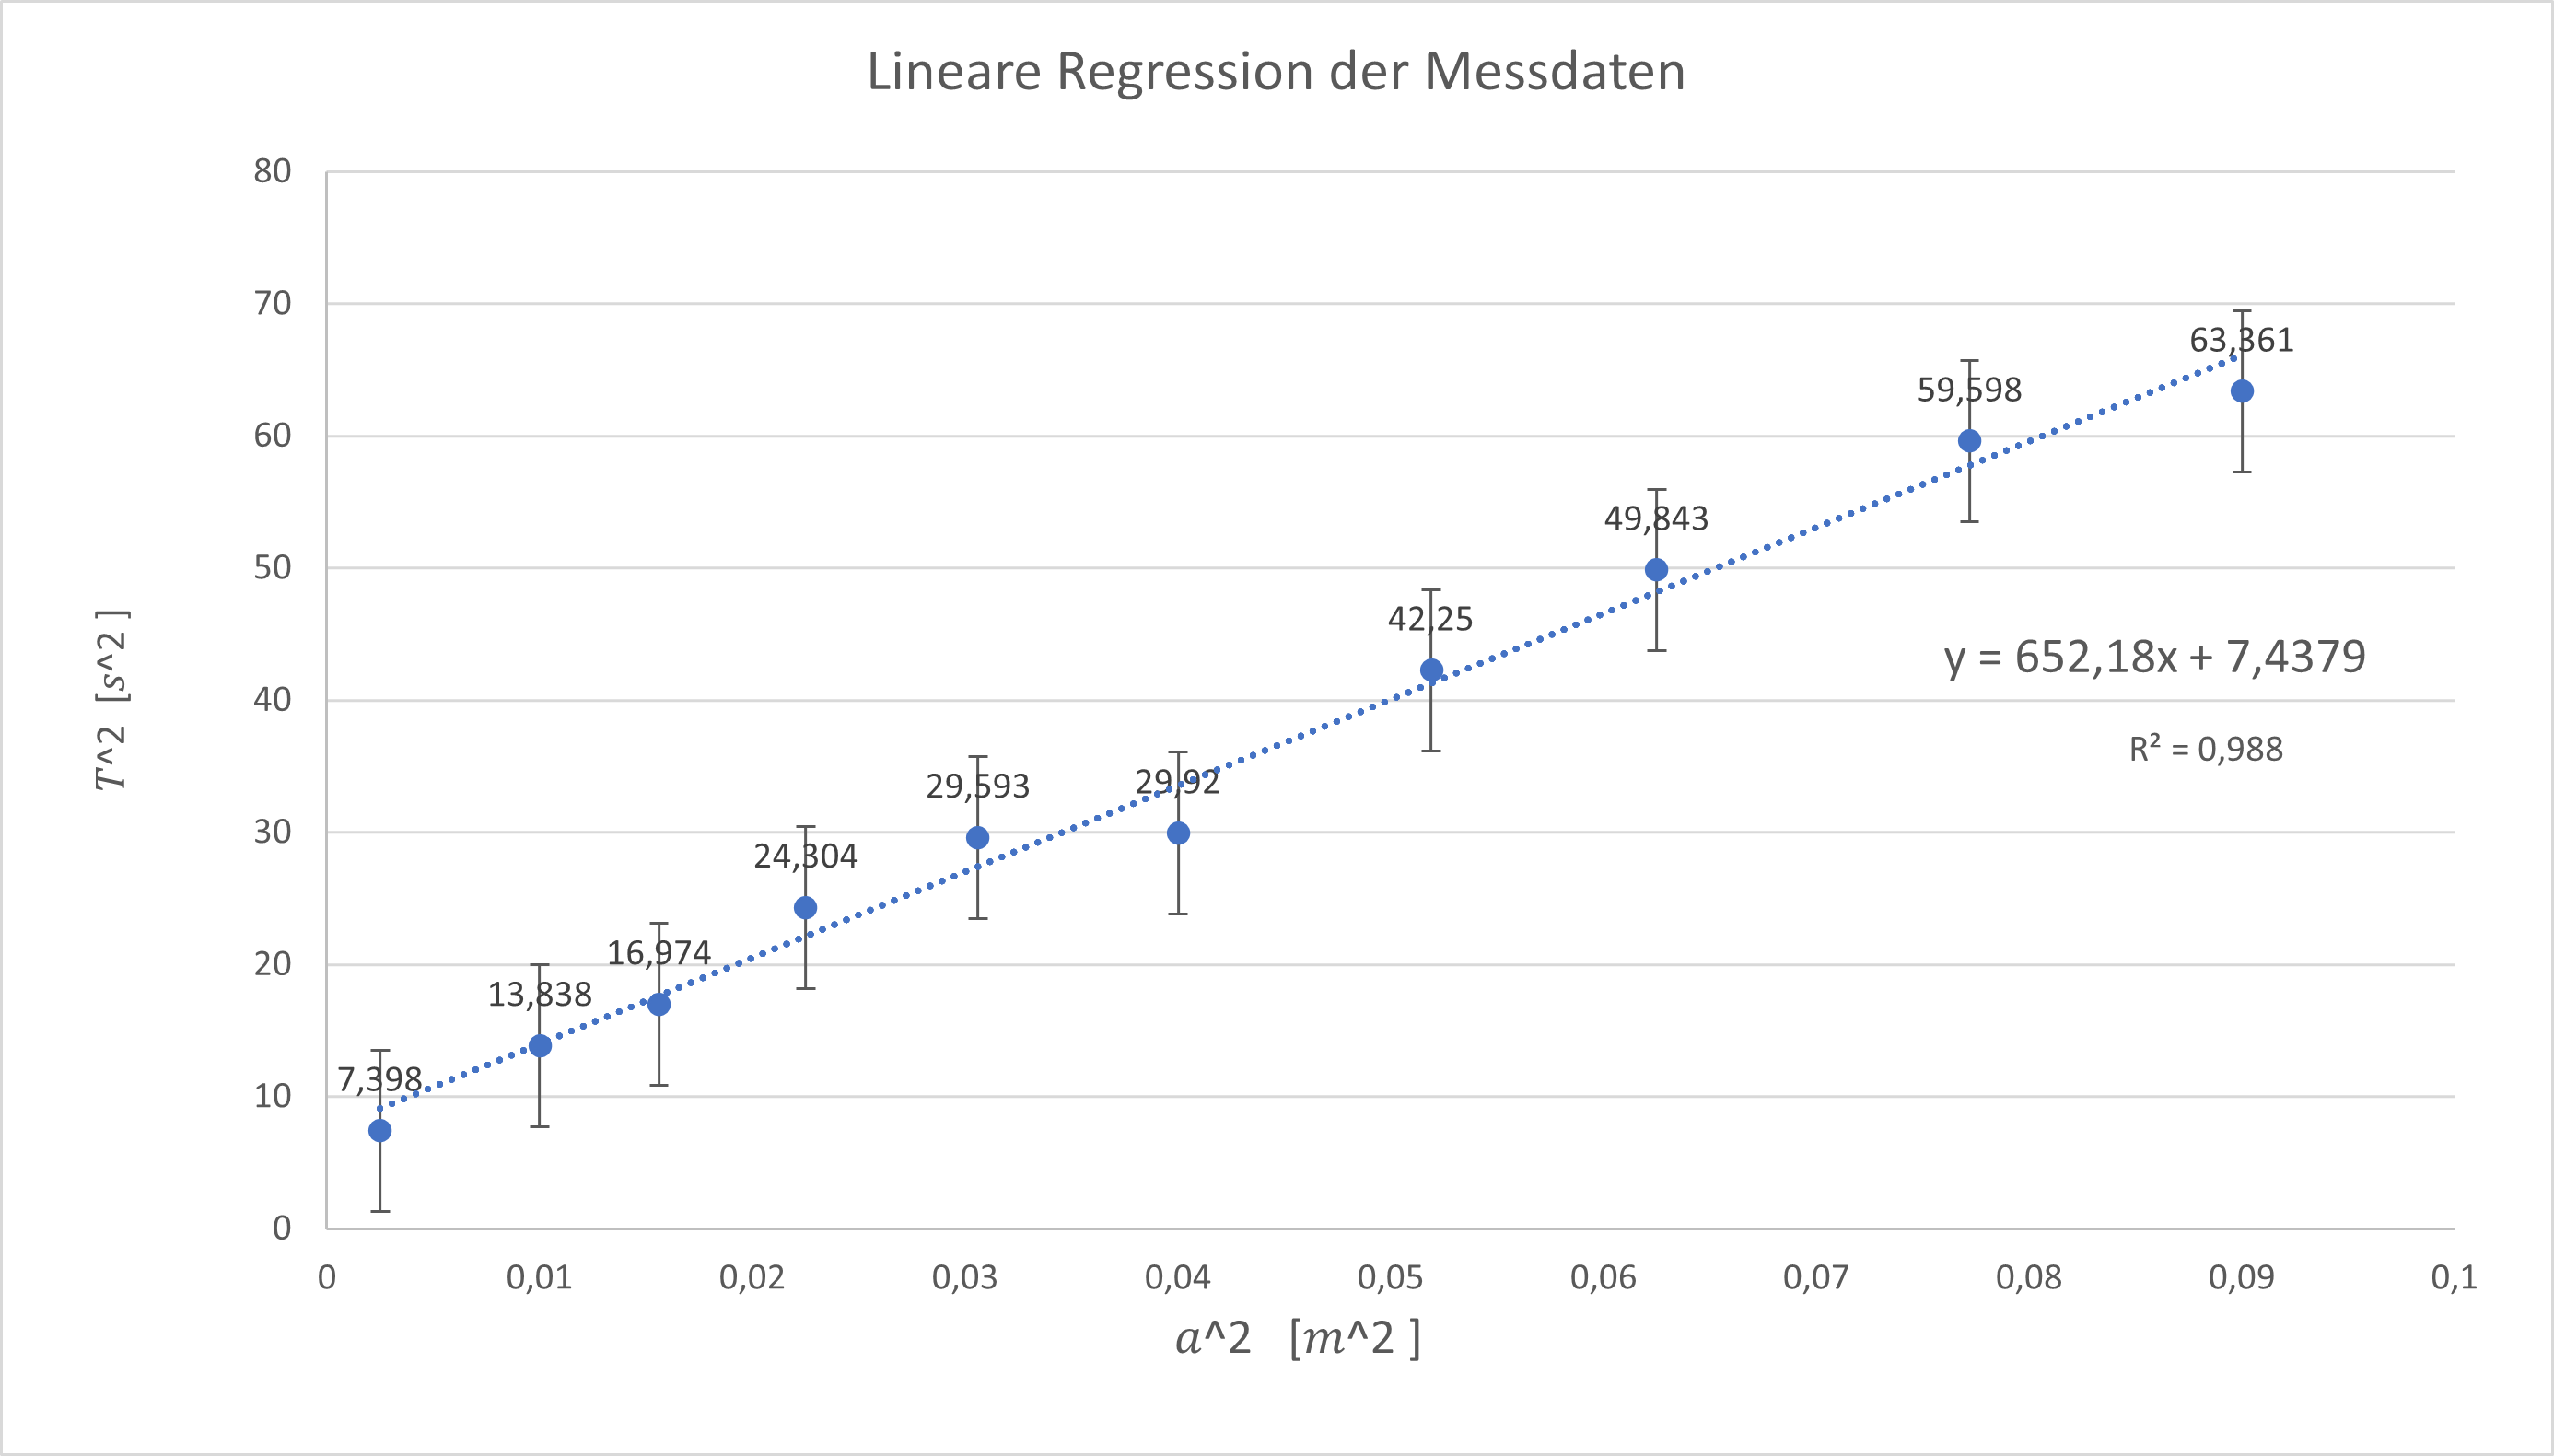
\includegraphics[height=60mm]{bilder/linearereg.png}
    \caption{Die lineare Regression verbildlicht. \label{Abbildung6}}
\end{figure}

\begin{flushleft}
    Es folgt daraus: 
\end{flushleft}

\begin{align*}
     r^2 = 0,98799565112239  \\
     r = 0,9959797035792  \\
     m = 652,183\, \unit{\second^2\meter^2} \\
     \increment m = 25,416\, \unit{\second^2\meter^2}  \\
     b = 7.4379\,\unit{\second^2}  \\
     \increment b = 1,2464\,\unit{\second^2}   \\
\end{align*}

\noindent{mit GTR (Grafikfähiger Taschenrechner) (\ref{Abbildung7})}:



\begin{align*}
    m = (652,183 \pm 25,416)\,\unit{\second^2\meter^2}\,\,\,\,\,\,b = (7,4379 \pm 1,2464) \unit{\second^2} 
\end{align*}

\noindent{mit}

\begin{center}
    \begin{align*}
        I_{D} = \frac{6 \cdot D}{4\pi^2} - 2 \cdot m_{D} \cdot \left(\frac{r_{D}^2}{4} + \frac{h_{D}^2}{12}\right) {D}  \\
        = \frac{7,4379 \unit{\second^2}  \cdot 0,0231 \unit{\newton\meter}}{4\pi^2} - 2 \cdot 0,2612 \unit{\kilogram} \cdot \left(\frac{(0,0225\unit{\meter})^2}{4}  +  \frac{(0,028\unit{\meter})^2}{12}  \right) \\
        =4,25 \cdot 10^{-3}\, \unit{\kilogram\meter^2} = 0,00425\, \unit{\kilogram\meter^2} 
    \end{align*}
\end{center}

\begin{figure}
    \centering
    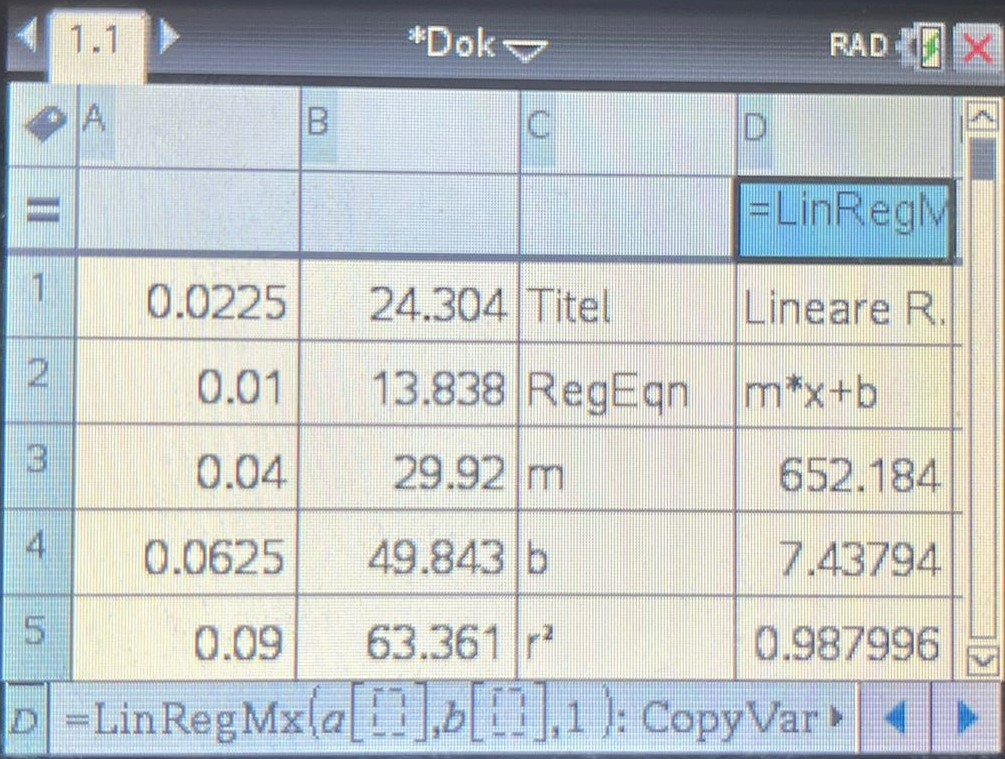
\includegraphics[height=50mm]{bilder/gtr.jpeg}
    \caption{Die lineare Regression mit dem Grafikfähigen Taschenrechner. \label{Abbildung7}}
\end{figure}

\begin{flushleft}
    Fehlerfortpflanzung:
\end{flushleft}

\begin{align*}
    \increment I_{D} = \sqrt{  \left(\frac{b}{4\pi^2}\right)^2 \cdot (\increment D)^2 + \left(\frac{D}{4\pi^2}\right)^2 \cdot (\increment b)^2 } \\
    = \sqrt{  \left(\frac{7,4379\unit{\second^2}}{4\pi^2}\right)^2 \cdot (0,001851)^2 + \left(\frac{0,0231 \,\unit{\newton\meter}} {4\pi^2}\right)^2 \cdot (1,2464)^2 } \\
    I_{D} = (0,00425 \pm 0.00131 )\, \unit{\kilogram\meter^2}
\end{align*}

\begin{table}
    \centering
    \caption{Messdaten für das Eigenträgheitsmoment}
    \label{Tabelle2}
    \begin{tabular} {c  c  c  c}
        \toprule
        {$a  \mathbin{/}  \unit{\meter} $} &
        {$a^{2}  \mathbin{/}  \unit{\meter^{2}}$} &
        {$T  \mathbin{/}  \unit{\second}$} &
        {$T^{2}  \mathbin{/}  \unit{\second}^2$} \\
        \midrule
        \vspace{0.2cm}
        0,05  & 0,0025 & 2,72 &  7,398 \\
        \vspace{0.2cm}
        0,10  & 0,01   & 3,72 & 13,838 \\
        \vspace{0.2cm}
        0,125 & 0,0156 & 4,12 & 16,974 \\
        \vspace{0.2cm}
        0,15  & 0,0225 & 4,93 & 24,304 \\
        \vspace{0.2cm}
        0,175 & 0,0306 & 5,44 & 29,593 \\
        \vspace{0.2cm}
        0,20  & 0,04   & 5,47 & 29,920 \\
        \vspace{0.2cm}
        0,228 & 0,0519 & 6,50 & 42,250 \\
        \vspace{0.2cm}
        0,25  & 0,0625 & 7,06 & 49,843 \\
        \vspace{0.2cm}
        0,278 & 0,0772 & 7,72 & 59,598 \\
        \vspace{0.2cm}
        0,30  & 0,09   & 7,96 & 63,361 \\
        \bottomrule
    \end{tabular} 
\end{table}


\begin{flushleft}
    Die Werte für die Bestimmung des Trägheitsmoments des Zylinders lauten:
\end{flushleft}

\begin{align*}
     r_{Z1} = 4,8\, \unit{\centi\meter} = 0.048\, \unit{\meter} \\
     h_{Z1} = 0,10016\, \unit{\meter}  \\
      m_{Z1} = 0,3675\, \unit{\kilogram}  \\
\end{align*}

\begin{align*}
     \intertext{\underline{Theoretisch}}  
     I_{Zl,\text{Theo}}= \frac{1}{2}mR^2 = \frac{1}{2} \cdot 0,3675\,\unit{\kilo\gram} \cdot (0,0048\,\unit{\meter})^2 = 4,23 \cdot 10^{-4}\,\unit{\kilo\gram\meter^2}   \\
\end{align*}


\begin{flushleft}
    \underline{Experimentell}: \quad
    $ \alpha = 180 \unit{\degree} $
\end{flushleft}


\begin{table}
    \centering
    \caption{Messdaten Trägheitsmoment Zylinder}
    \label{Tabelle3}
    \begin{tabular} {c}
        \toprule
        {$ T_{\text{Zylinder}} \mathbin{/} \unit{\second} $} \\
        \midrule
        0,66 \\
        0,75 \\
        0,86 \\
        0,68 \\
        0,78 \\
    \end{tabular} 
\end{table}

\begin{center}
   mit den Werten aus der Tabelle folgt: \quad $ \bar{x} = 0,744\, \unit{\second}$ \\
   mit $  \sigma = 0,078 $ \quad \to \quad $ T_{Z1,Exp} = (0,744 \pm 0,078)\, \unit{\second} $\\
\end{center}
\begin{align*}
   \intertext{Trägheitsmoment:} 
   I = \frac{T^2 \cdot D}{4\pi^2} = \frac{(0,744 \unit{\second})^2 \cdot 0,0231 }{4\pi^2} = 0,000323\, \unit{\kilo\gram} \cdot \unit{\meter^2}
\end{align*}

\newpage

\begin{flushleft}
    Fehlerfortpflanzung:
\end{flushleft}


\begin{align*}
    \increment K1 = \sqrt{ \left(\frac{2\cdot D\cdot T_{Z1}}{4\pi} \right)^2 \cdot (\increment T_{Z1})^2 + \left(\frac{T_{Z1}}{4\pi} \right)^2 \cdot (\increment D)^2} \\
    = \sqrt{ \left(\frac{2\cdot 0,0231 \cdot 0,744\unit{\second}}{4\pi} \right)^2 \cdot (0,078\unit{\second})^2 + \left(\frac{0,744}{4\pi} \right)^2 \cdot (0,001851)^2 } = 0,00022\,\unit{\kilo\gram\meter^2}  \\
\end{align*}


\begin{center}
    somit ergibt sich \to $ I_{Z1} = (0,000323 \pm 0,00022)\,\unit{\kilo\gram\meter^2} $
\end{center}

\begin{flushleft}
    Die Werte für die Bestimmung der Trägheits der Holzkugel lauten:
\end{flushleft}

\begin{align*}
 r_{K2} = 0,0702\, \unit{\meter}  \\
 d_{K2} = h_{Z2} = 0,1404\, \unit{\meter}  \\
 m_{K2} = 1,1725\, \unit{\kilogram}  \\
\end{align*}


\begin{table}
    \centering
    \caption{Messdaten Trägheitsmoment Zylinder}
    \label{Tabelle4}
    \begin{tabular} {c}
        \toprule
        {$ T_{K2} \mathbin{/} \unit{\second} $} \\
        \midrule
        1,85 \\
        1,59 \\
        1,75 \\
        1,75 \\
        1,88 \\
        \bottomrule
    \end{tabular} 
\end{table}

\begin{center}
    durch die Werte aus der Tabelle folgt : \quad $ \bar{x} = 1,764\, \unit{\second} $ \\
    mit $  \sigma = 0,1134 $ \quad \to \quad $ T_{K2,Exp} = (0,744 \pm 0,078)\, \unit{\second}   $
    
    \vspace{0.3cm}
 
    Trägheitsmoment: $ I = \frac{(1.764 \unit{\second})^2 \cdot (0,0231) }{4\pi^2} = 0,00182\,\unit{\kilo\gram}\cdot\unit{\meter^2} $ \\

    \vspace{0.5cm}

    $ \increment I = \sqrt{ \left(\frac{2\cdot (0,0231) \cdot 1,764\unit{\second}}{4\pi} \right)^2 \cdot (0,1134)^2 + \left(\frac{1,764^2\unit{\second}}{4\pi} \right)^2 \cdot (0,001851)^2 } = 0,000866\,\unit{\kilogram\meter^2} $ \\

    \vspace{0.5cm}

    \underline{$ I_{K2, Exp} = (0,00182 \pm 0,000866)\,\unit{\kilogram\meter^2} $ }

    \vspace{0.5cm}

    \underline{Theoretisch}: $ \frac{2}{5}mR^2 = \frac{2}{5} 1,1725\, \unit{\kilogram} \cdot (0,0702 \,\unit{\meter})^2 = 2,311 \cdot 10^{-3\,} \unit{\kilogram\meter^2}  $
\end{center}


\begin{flushleft}
    Die Holzpuppe hat eine Masse von $ m_{p} = 0,1675\, \unit{\kilogram} $
\end{flushleft}

\begin{table}
    \centering
    \caption{Messdaten der Radien der Holzpuppe}
    \label{Tabelle5}
    \begin{tabular} {c  c  c  c}
        \toprule
        {$r_{\text{Rumpf}} \mathbin{/} \unit{m}$} &
        {$r_{\text{Arm}}   \mathbin{/} \unit{m}$} &
        {$r_{\text{Bein}}  \mathbin{/} \unit{m}$} &
        {$r_{\text{Kopf}}  \mathbin{/} \unit{m}$} \\
        \midrule
        \vspace{0.2cm}
        0,03912& 0,014 & 0,019   & 0,023    \\
        \vspace{0.2cm}
        0,026  & 0,138 & 0,016   & 0,027    \\
        \vspace{0.2cm}
        0,032  & 0,012 & 0,0121  & 0,02708  \\
        \vspace{0.2cm}
        0,0386 & 0,014 & 0,01706 & 0,025    \\
        \vspace{0.2cm}
        0,040  & 0,013 & 0,13    & 0,0211   \\
        \vspace{0.2cm}
        0,038  & 0,016 & 0,009   & 0,02812  \\
        \bottomrule
    \end{tabular} 
\end{table}

\newpage 

\begin{center}
    durch das mitteln der Radien folgen die Werte: \\
    \begin{align*}
        r_{\text{Rumpf}} = (0,03562\pm 0,0055)\, \unit{\meter} \\
        r_{\text{Arm}} = (0,0138 \pm 0,0013)\, \unit{\meter}  \\
        r_{\text{Bein}} = (0,01436 \pm 0,0036)\, \unit{\meter}  \\
        r_{\text{Kopf}} = (0,0253 \pm 0,0028)\, \unit{\meter}  \\
    \end{align*}

    hierbei sind die Werte  $\bar{x} $ und die Messunsicherheiten $\sigma$ 

    \vspace{0.3cm}

    Die Länge der einzelnen Teile des Holzpuppe betragen:\\
    
    \begin{align*}
    L_{\text{Rumpf}} = 0,0918\, \unit{\meter} \\
    L_{\text{Arm}} = 0,112\, \unit{\meter} \\
    L_{\text{Bein}} = 0,147\, \unit{\meter} \\
    L_{\text{Kopf}} = 0,041\,\unit{\meter} \\
    \end{align*}
\end{center}

\begin{center}
    Alle Körperteile werden als Zylinder betrachtet: \\

    \vspace{0.3cm}

    $V_{\text{Zylinder}} = \pi r^2 L $   und $ \increment V_{\text{Zylinder}} =\sqrt{\left( 2 \pi \cdot L_{\text{Koerperteil}} \cdot r_{\text{Koerperteil}}\right)^2 \cdot \left(\increment r_{\text{Koerperteil}}\right)^2} $

    \begin{align*}
     V_{\text{Rumpf}} = (3,65 \pm 0,13)\, \cdot 10^{-4}\,\unit{\meter^3}  \\
     V_{\text{Arm}} = (0,067 \pm 0,0126)\, \cdot 10^{-4}\,\unit{\meter^3}  \\
     V_{\text{Bein}} = (0,095 \pm 0,047)\, \cdot 10^{-4}\,\unit{\meter^3}  \\
     V_{\text{Kopf}} = (0,082 \pm 0,01)\,  \cdot 10^{-4}\,\unit{\meter^3}  \\
    \end{align*}
\end{center}

\begin{center}
    \begin{align*}
     \increment V_{\text{ges}} = \sqrt{(\increment V_{\text{Rumpf}})^2 + 4 \cdot (\increment V_{\text{Arm}})^2 +4 \cdot (\increment V_{\text{Bein}})^2 + (\increment V_{\text{Kopf}})^2}  \\
     V_{ges} = (0,000609 \pm 0,00016)\, \unit{\meter^3} \\
    \end{align*}

    Teilvolumina am Gesamtvolumen: \\ 

   

    $ A_{\text{Koerperteil}} = \frac{V_{\text{Koerperteil}}}{V_{\text{ges}}} $ \\

    \vspace{0.3cm}

    mit der dazugehörigen Fehlerfortpflanzung: \\

    \vspace{0.3cm}

    $ \increment A_{\text{Koerperteil}} = \sqrt{ \left(\frac{1}{V_{\text{ges}}}\right)^2 \cdot (\increment V_{\text{Koerperteil}})^2 + \left( -\frac{V_{\text{Koerperteil}}}{V_{\text{ges}}}^2  \right)^2 \cdot (\increment V_{\text{ges}})^2}$

    \vspace{0.7cm}

    \underline{Anteile} \\    

    \begin{align*}
     A_{\text{Rumpf}} = (0,599 \pm 0,265)   \\
     A_{\text{Arm}}   = (0,11 \pm 0,0350)   \\
     A_{\text{Bein}}  = (0,159 \pm 0,0786)  \\
     A_{\text{Kopf}}  = (0,1346 \pm 0,039)  \\
    \end{align*}

    $ m_{\text{Koerperteil}} = A_{\text{Koerperteil}} \cdot m_{\text{Puppe}} $ \\

    \begin{align*}
     m_{\text{Rumpf}} = 0,1003\, \unit{\kilogram}  \\
     m_{\text{Arm}} = 0,0183\, \unit{\kilogram}  \\ 
     m_{\text{Bein}} = 0,0266\, \unit{\kilogram}  \\
     m_{\text{Kopf}} = 0,0225\, \unit{\kilogram}  \\
    \end{align*}
\end{center}

\newpage

\begin{flushleft}
    Die Theoretischen Werte für die Trägheit der ersten Haltung setzen sich zusammen aus, \\
    dem Trägheitsmoment des Rumpfes und des Kopfes aus der Formel (\ref{4}), sowie für die Arme und Beine
    aus den Formeln (\ref{2}) und (\ref{4}), mit Hilfe des Satzes von Steiner.
\end{flushleft}

\begin{align*}
 I_{\text{Arm}} = \frac{m_{\text{Arm}} \cdot r^2_{\text{Arm}}}{2} + m_{\text{Arm}} \cdot (r_{\text{Rumpf}} + r_{\text{Arm}})^2 \\
 I_{\text{Bein}} = \frac{m_{\text{Bein}} \cdot r^2_{\text{Bein}}}{2} + m_{\text{Bein}} \cdot r^2_{\text{Bein}}   \\
 \increment I_{\text{Koerperteil}} = \sqrt{(m_{\text{Koerperteil}} \cdot r_{\text{Koerperteil}})^2 \cdot (\increment r_{\text{Koerperteil}})^2 } \\
 \increment I_{\text{Arm}} = \sqrt{ (m_{\text{Arm}} \cdot(2r_{\text{Arm}} + 3r_{\text{Rumpf}}))^2 \cdot (\increment r_{\text{Arm}})^2 } \\
 \increment I_{\text{Bein}} = \sqrt{ (m_{\text{Bein}} \cdot r_{\text{Bein}} \cdot (1+r_{\text{Bein}}))^2 \cdot (\increment r_{\text{Bein}})^2 }\\
 I_{Zi(\text{Kopf/Rumpf})} = \frac{1}{2}mR^2 
\end{align*}

Gesamtfehler:  $ \increment I_{Puppe} = \sqrt{(\increment I_{Rumpf})^2 + 4(\increment I_{Arm})^2 +4(\increment I_{Bein})^2 + (\increment I_{\text{Koerperteil}})^2} $ \\
    
\begin{align*}
 I_{\text{Kopf}} = 7,2 \cdot 10^{-6}\,\unit{\kilo\gram\meter^2}  \\
 I_{\text{Rumpf}} = 6,36 \cdot 10^{-5}\,\unit{\kilo\gram\meter^2}  \\
 I_{\text{Arm}} = 7,87 \cdot 10^{-11}\,\unit{\kilo\gram\meter^2}   \\
 I_{\text{Bein}} = 8,22 \cdot 10^{-6}\,\unit{\kilo\gram\meter^2}  \\
 \increment I_{\text{Kopf}} = 3,21 \cdot 10^{-6}\,\unit{\kilo\gram\meter^2}  \\
 \increment I_{\text{Rumpf}} = 1,39 \cdot 10^{-6}\,\unit{\kilo\gram\meter^2}  \\
 \increment I_{\text{Arm}} = 1,5939 \cdot 10^{-6}\,\unit{\kilo\gram\meter^2}  \\
 \increment I_{\text{Bein}} = 1,96 \cdot 10^{-5}\,\unit{\kilo\gram\meter^2}  \\
\end{align*}

durch mitteln folgt der Wert  $ \increment I_{\text{Puppe}} = 2,087 \cdot 10^{-5}\,\unit{\kilo\gram\meter^2} $\\
\begin{align*}
    I_{\text{Theo,Puppe}} = (7,9 \cdot 10^{-5} \pm 2,087 \cdot 10^{-5})\, \unit{\kilogram\meter^2} 
\end{align*}

\begin{flushleft}     
    \underline{Experimentelle Bestimmt}: \to $ \alpha = 90 \unit{\degree} $
\end{flushleft}

\begin{table}
    \centering
    \caption{Messdaten der Holzpuppe Haltung 1}
    \label{Tabelle6}
    \begin{tabular} {c}
        \toprule
        {$ T_{\text{Holzpuppe,1}} \mathbin{/} \unit{\second} $} \\
        \midrule
        0,32 \\
        0,31 \\
        0,35 \\
        0,44 \\
        0,34 \\
        \bottomrule
    \end{tabular} 
\end{table}

\begin{align*}
     \bar{x} = 0,352 \, \, \text{und}\, \,  \sigma = 0,0516  \to \,\,T = (0,352 \pm 0,0516)\, \unit{\second}  \\
     I_{H1} = \frac{T^2 \cdot D}{(2\pi)^2} = \frac{(0,352\, \unit{\second})^2 \cdot 0,0231}{(2\pi)^2} = 0,0000724\,\unit{\kilo\gram\meter^2} \\
     \increment I_{H1} = 0,0000692\,\unit{\kilo\gram\meter^2}   \\
     I_{H1} = ( 0,0000692 \pm 0,0000692 )\, \unit{\kilogram\meter^2}  
\end{align*}

\newpage

\begin{flushleft}
    Der Theoretisch ermittelte Wert für die zweite Haltung setzt sich zusammen aus, dem Satz von Steiner
    mit den Formeln (\ref{2}) und $ I_{\text{Stab}} = \frac{ml^2}{3} $ (Trägheitsmoment eines Stabes an den Enden)
    für die Arme. Mit der Formel (\ref{4}) für den Rumpf und dessen Kopf, sowie (\ref{2}) und (\ref{4}) für die Beine.
\end{flushleft}

\begin{align*}
     I_{\text{Arm}} = \frac{m_{\text{Arm}} \cdot L^2_{\text{Arm}}}{3} + m_{\text{Arm}} \cdot r^2_{\text{Rumpf}} = 1,002 \cdot 10^{-4}\,\unit{\kilogram\meter^2} \\
     I_{\text{Rumpf}} = \frac{1}{2}m_{\text{Rumpf}} \cdot R^2_{\text{Rumpf}} = 6,36 \cdot 10^{-5}\,\unit{\kilogram\meter^2} \\
     I_{\text{Kopf}} = \frac{1}{2}m_{\text{Kopf}} \cdot R^2_{\text{Kopf}} = 7,2 \cdot 10^{-6}\,\unit{\kilogram\meter^2} \\
     I_{\text{Bein}} = \frac{m_{\text{Bein}} + r^2_{\text{Bein}}}{2} + m_{\text{Bein}} \cdot r^2_{\text{Bein}} = 8,22 \cdot 10^{-6}\,\unit{\kilogram\meter^2} \\
     I_{\text{Arm}} = \sqrt{ (2m_{\text{Arm}} \cdot r_{\text{Rumpf}}) \cdot (\increment r_{\text{Rumpf}})^2} = 1,99 \cdot 10^{-4}\,\unit{\kilogram\meter^2}  \\
     \increment I_{\text{Bein}} = 1,39 \cdot 10^{-6}\,\unit{\kilogram\meter^2}  \\
     \increment I_{\text{Kopf}} = 1,59 \cdot 10^{-6}\,\unit{\kilogram\meter^2}  \\
     \increment I_{\text{Rumpf}} = 1,96 \cdot 10^{-6}\,\unit{\kilogram\meter^2}   \\
     I_{Theo,H2} = (0,000179 \pm 0,000398)\, \unit{\kilogram\meter^2} 
\end{align*}


\begin{table} 
    \centering
    \caption{Messdaten der Holzpuppe Haltung 2}
    \label{Tabelle7}
    \begin{tabular} {c}
        \toprule
        {$ T_{\text{Holzpuppe,2}} \mathbin{/} \unit{\second} $} \\
        \midrule
        0,50 \\
        0,60 \\
        0,44 \\
        0,44 \\
        0,53 \\
        \bottomrule
    \end{tabular} 
\end{table}

\begin{center}
    $\bar{x} = 0,502$ \,\,\,  und \,\,\, $\sigma = 0,067 $
\end{center}

\begin{align*}
    \to  \,  T_{H2} = (0,502 \pm 0,067)\, \unit{\second}\\
    I_{H2} = \frac{T^2 \cdot D}{4\pi^2} = \frac{(0,5020 \unit{\second})^2 \cdot 0,0231}{4 \pi^2} = 1,47 \cdot 10^{-4}\,\unit{\kilogram\meter^2} \\ 
    \increment I_{H2} = 0,000129\,\unit{\kilogram\meter^2} \\
    I_{H2,Exp} = (0,000147 \pm 0,000129)\,\unit{\kilogram\meter^2} 
\end{align*}
